\subsection{Seguimiento}

El seguimiento de trayectorias se realiza sobre una ventana deslizante de tres a cuatro cuadros donde se enlazan los puntos reconstruidos de manera de mantener un movimiento lo mas suave posible.

Esta metodología fue la utilizada por Herda \cite{herda} en su trabajo basándose en los estudios de Malik, Drako, Papantoniou \cite{griegos} .

%\subsubsection{Algoritmo}
\hspace*{0.5cm} \textit{Algoritmo.} Sea la trayectoria de un marcador enlazada hasta el instante [f] sobre la cual desea buscarse su próximo punto en [f+1], el movimiento entre [f-1] y [f] es prolongado para establecer un centro de búsqueda y encontrar el punto reconstruido que mejor continúa la trayectoria como se muestra en la Figura \ref{herda_00} .

\vspace{-0.7cm}
\begin{figure}[ht!]
\begin{center}
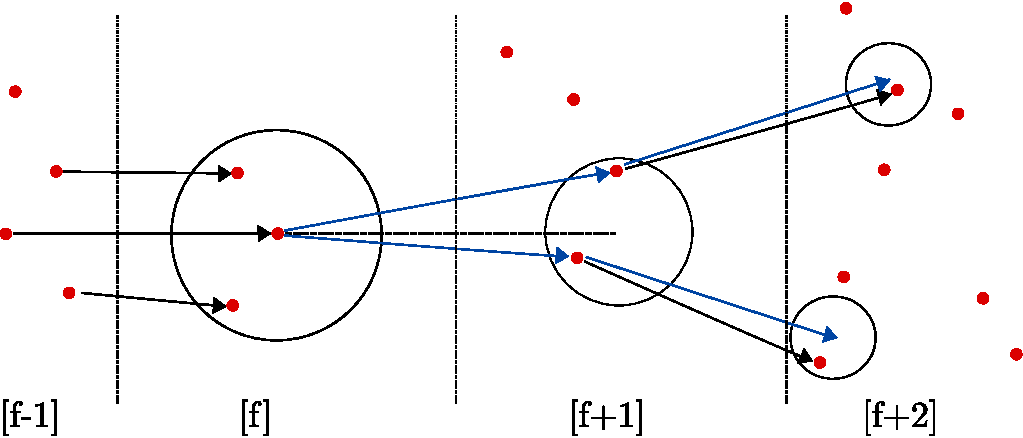
\includegraphics[scale=0.4]{imagenes/Seguimiento/tracking-eps-converted-to.pdf}
\end{center}
\caption{Seguimiento en cuatro cuadros, siendo [f] el cuadro actual que queremos seguir en [f+1]. ( Fuente  Human movement
science 20(3), 313–341 \cite{herda} ) .}
\label{herda_00}
\end{figure}
\vspace{-0.3cm}
Se presentan tres posibles casos al buscar puntos reconstruidos:

\begin{itemize}

\item Si solo se encuentra un punto reconstruido se agrega a la trayectoria para el cuadro [f+1], buscando el mas cercano a la estimación calculada como aquella que mejor se aproxima a una trayectoria de tres puntos con aceleración mínima

\item En el caso de encontrar mas de un punto cada posible candidato es evaluado para realizar una segunda estimación hacia [f+2] de forma que la aceleración entre [f-1], [f] y el candidato en [f+1] sea la misma que entre [f], el candidato en [f+1] y la estimación en [f+2]. Luego de todos los posible caminos en cuatro cuadros, se elige el de menor variación de aceleración.

\item Si no se encuentra ningún punto, se procede a aumentar de forma limitada el radio de búsqueda en [f+1] de forma excepcional. Esto se hace para continuar trayectorias que entran en estado de reposo y el último movimiento conocido es nulo o muy pequeño.

\end{itemize}

Si una trayectoria queda trunca durante el enlazado, se intenta recuperar prolongando el movimiento en próximas cuadros para encontrar puntos reconstruidos cercanos a las estimaciones y extrapolar los puntos intermedios. Por otro lado, se implementan umbrales para definir límites sobre la aceleración de los enlaces obtenidos y detectar discontinuidades durante el seguimiento.

Con estas medidas implementadas es posible detectar las trayectorias individuales sobre los puntos reconstruidos, detectar de forma simple posibles discontinuidades, y estimar reemplazos en casos de pérdidas. La captura mostrada en la Figura \ref{restricciones_tracking} corresponde a la marcha y se resaltan las trayectorias individuales de puntos de la pierna así como un esqueleto simple generado simplemente para visualizar la evolución entre marcadores
\vspace{-0.25cm}
\begin{figure}[ht!]
 \begin{center}
%  \subfloat[Trayectorias de marcadores de pierna]
  {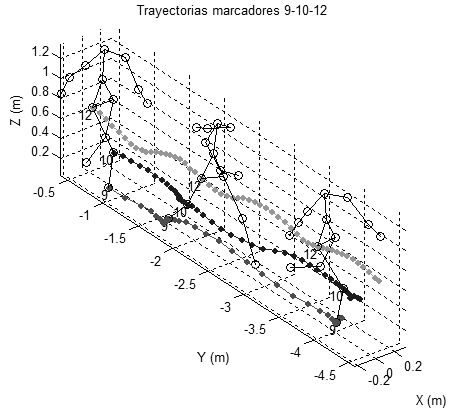
\includegraphics[scale=0.4]{imagenes/Seguimiento/050_Salida_Tracking_13_14_10.png} %\label{trayectorias_marcadores_piernas}
   }	
 % \subfloat[Distancia y Angulo entre marcadores de la pierna.]
 {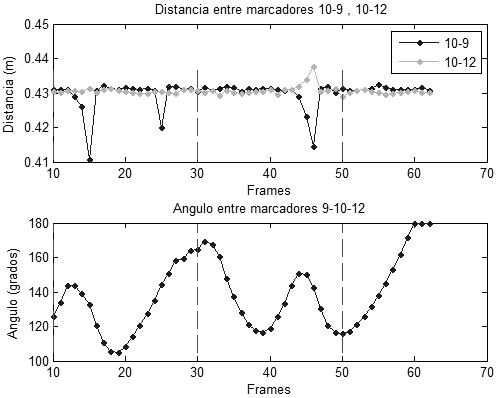
\includegraphics[scale=0.4]{imagenes/Seguimiento/051_Salida_Angulo_Distancia_13_14_10.png}\label{distancia_angulo_marcadores_piernas}}
  \end{center}
\caption{Posibles restricciones en ángulo y distancia, para el caso de la pierna en marcha. Izquierda: trayectorias de marcadores de pierna. Derecha: distancia y ángulo entre marcadores de la pierna.}
\label{restricciones_tracking}
\end{figure}
\vspace{-0.5cm}

El conjunto de puntos reconstruidos puede ser sometido a otros algoritmos de seguimiento como por Kalman \cite{kalman} requiriendo la inicialización de modelos, o algoritmos basados en restricciones mas fuertes a las presentadas en este trabajo como podrían ser las distancias relativamente constantes entre marcadores de los miembros y ángulos continuos entre articulaciones, pero requieren un estudio considerable de las características de cada sujeto y movimiento a capturar. La Figura \ref{restricciones_tracking} muestra algunas posibles restricciones en la marcha sobre los huesos de la pierna.

